\begin{figure}
\centering
\pandocbounded{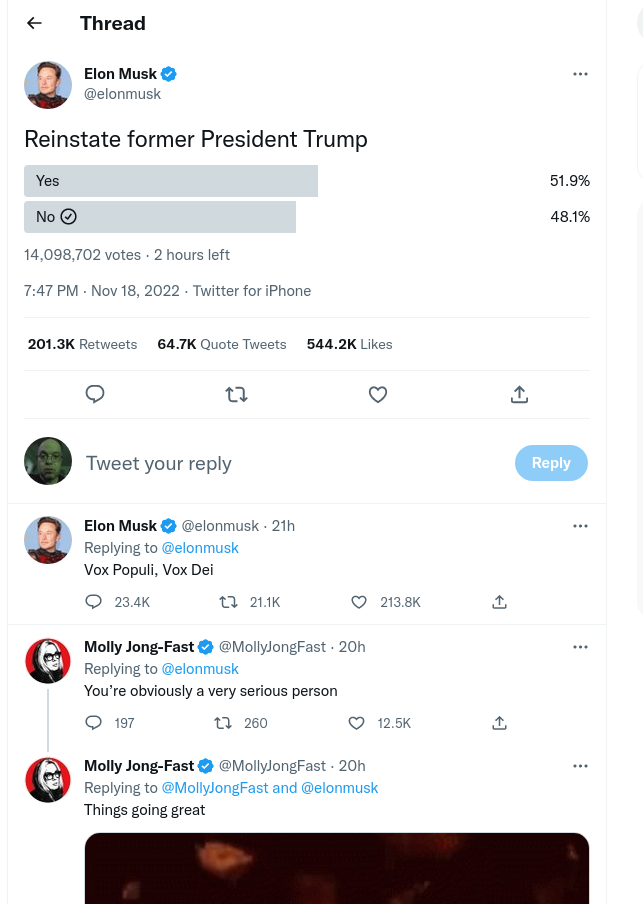
\includegraphics[keepaspectratio]{\%7B\%7Bsite.url\%7D\%7D/img/MuskCrazyIdea.png}}
\caption{Clipped screenshot of a poll on Twitter run by Elon Musk
concerning reinstating Donald John Trump to the platform}
\end{figure}

Well, that's frankly rather disturbing. Mr.~Musk really wants to appeal
to a core audience of craziness. Keeping the Trump dream alive
definitely resonates with part of the economy, perhaps. It is part of
the economy I truly do not want to take part in. The former president
has done so many wild things that the Justice Department brought in a
former war crimes prosecutor who handled cases \emph{from Kosovo} to
handle the January 6th and classified documents investigations. Wouldn't
a reasonable person think that perhaps that's a clue that we may be
dealing with a supervillain here?

That screenshot was from the middle of the afternoon on Saturday. Later
on Saturday this popped up on my Apple Watch:

\begin{figure}
\centering
\pandocbounded{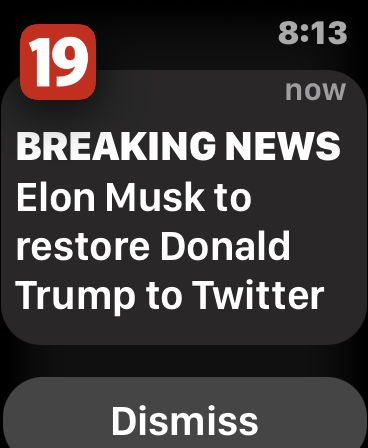
\includegraphics[keepaspectratio]{\%7B\%7Bsite.url\%7D\%7D/img/trump-restored-twitter.png}}
\caption{Screenshot from watchOS of a notification from the Cleveland19
app indicating that Donald Trump is seeing his ban from Twitter being
rescinded}
\end{figure}

We're seeing bad things happen now!
